%!TEX TS-program = lualatex
%!TEX encoding = UTF-8 Unicode

%\frame[plain]{ % When including a large figure or table, you don't want to have the bottom and the top of the slides.
%\frame[shrink]{ % If you want to include lots of text on a slide, use the shrink option.

\begin{frame}[shrink]
    \frametitle{FUSE (File System in User Space)}
    \begin{center}
        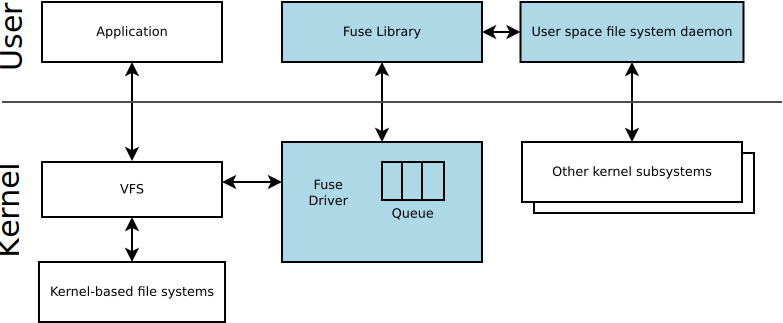
\includegraphics[width=1.2\textwidth]{frames/img/fuse_arch_new}
    \end{center}
    
    \begin{itemize}
        \item simplifies writing file system drivers by avoiding kernel-space code
        \item mounting / unmounting can be done as an unprivileged user and file system logic runs in user space process
    \end{itemize}
    
    \note{
    \begin{itemize}
        \item \textbf{SLOW: and ask:} First explain how FS works. For now, ignore the right side. Just look at the left column
        \item nowadays OSes divide their memory in user and kernel space and they use a feature system protection rings in PC to enforce it. \textbf{Above vertical line user, below kernel}
        \item So adding 5+5, userspace, reading from a file, syscall, kernel does the work delivers result back.
        \item  \textbf{LEFT SIDE}, read, VFS, then it will see what FS it is for, EXT4, read, read from disk, back, back to user
        \item kernel driver exposes a queue of requests to user space... \textbf{... which is consumed by a user space daemon handling those requests} => GO WHOLE WAY back and forth
        \item SAVE TIME, not re-implement, nice to re-use

    \end{itemize}
    }
\end{frame}